% !TEX root = ../Thesis.tex
\chapter{Feed Trees}

While feeds are a very powerful concept, there are still some limitations to them. Once a packet is appended it cannot be changed or replaced anymore (this would violate the append-only concept, see \cref{sec:signing}). It is not possible to start replicating the feed at any arbitrary packet position, it has to be built up starting with the header and appending packet after packet until the relevant position is reached (chain of trust, see \cref{sec:anchor}). Since a single feed alone cannot implement those features, we need a different solution. In this section we will explore how we can simulate the desired functionalities using the concepts discussed in \cref{sec:tiny} and some small additions to the TinySSB protocol. By using feeds, child feeds and continuation feeds as building blocks, larger structures can be constructed that are called 'feed trees'. The goal is that the user can interact with those trees on an abstract level as if it were feeds with added functionalities, while hiding the underlying technical complexity.

\section{Fork Tree}
\subsection{Feed Limitations}
If a user realizes that an already appended packet in a feed has an outdated or faulty payload, (s)he cannot revert the append process. A quick fix is to append a new packet to the feed, that informs the nodes to disregard or reinterpret said packet while evaluating it. However the packet stored on the device itself cannot be altered and the fix can only be applied, once the packet containing it has arrived at the node. It also means that newly deployed nodes that replicate the feed have to first receive and append the faulty packet before receiving the fix (chain of trust) even though the feed owner could have created the packet with the fix long before. If not only one but a series of packets have flaws, additionally to the problems stated before, storage would be needed for a lot of undesirable packets. In an autonomous environment especially with only low storage availability, this will be a problem. A different fix is to completely abandon the feed and resend every packet with the updated fixes. While solving the storage problem, it has the disadvantage of taking a lot of time and using the network for sending packets again that were already sent before. Both methods are not desirable and therefore a more efficient solution is presented in this section. 

\subsection{Initialization}
To address the problem of reverting to an earlier position in a feed, the feed structure named 'fork tree' is introduced. A new packet type 'make-fork-tree' is added to the other TinySSB packets. It has technically the same functionality as the make-child packet since it also creates a new feed and points to it. However the packet also triggers TinySSB to create a new fork tree construct. To initialize the tree, three operations have to be performed. First the feed that is pointed at by the make-fork-tree packet (also called root feed) is created. Secondly an additional child feed gets created by appending a make-child packet to the root feed. And thirdly a payload 48 packet gets appended to the root feed as a placeholder. It is used to make the scanning of a larger fork trees easier and could in future implementations be used to add additional meta data to the tree. A newly initialized fork tree can be seen in \cref{fig:fork1}.

\begin{figure}
\centering
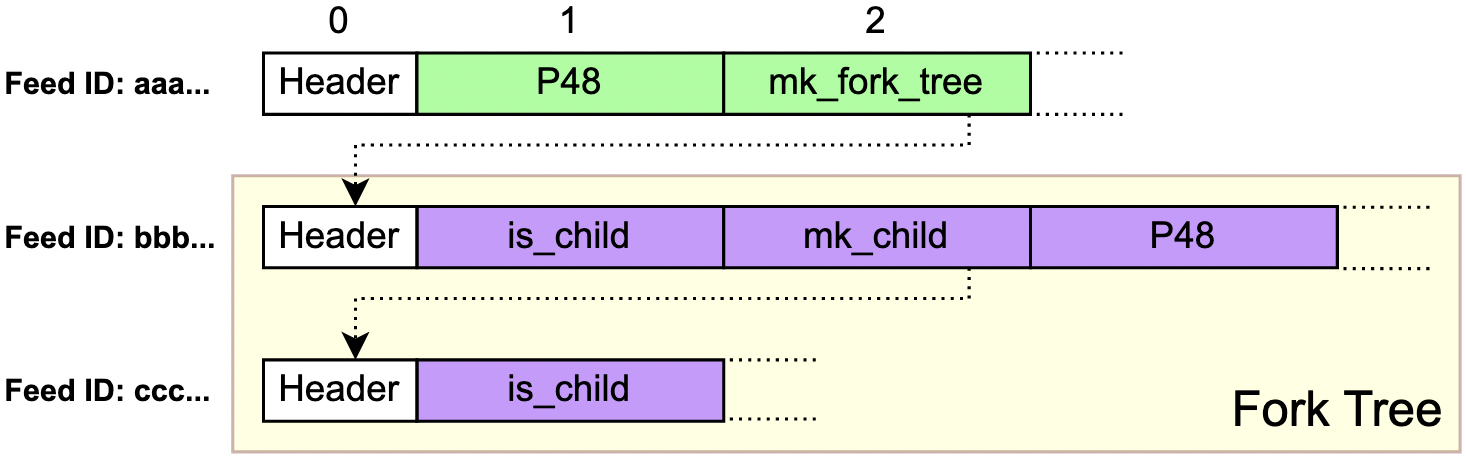
\includegraphics[width=1\textwidth]{fork1}
\caption{Second packet in feed aaa... initializes a new fork tree and points to root feed bbb... . The second packet in feed bbb... creates and points to feed ccc... .}
\label{fig:fork1}
\end{figure}
 
The child feed created from within the root feed is the emergency feed (feed ccc... in \cref{fig:fork1}). If at any point in the future a new fork needs to be created (see \cref{sec:forking}) the appropriate feed will already be present. After initialization the root feed of a fork tree is being used nearly identical to a normal feed. Any packet with either type payload 48 or chain 20 that the user appends to the tree will be automatically appended to the root feed. Other nodes that want to replicate the fork tree could theoretically replicate the initialized tree the same way they would replicate any other feeds and child feeds. However it is only after the structure gets more complex that a new solution must be found (see \cref{sec:dmxfork}).

\subsection{Creating a Fork}
\label{sec:forking}

The idea of creating forks is highly influenced from the ability to fork in version control systems[ADD SOURCE]. Creating a fork in a fork tree means to nominate any packet in the \textbf{packet chain}\footnote{A packet chain can be distributed over multiple feeds. It consists of only the payload packets manually appended by the user. When forking all packets newer than the fork packet are removed from the chain.} to be the new front packet of the tree. All packets that were appended later are disregarded and can even be discarded. Any further packet that gets appended to the tree continues directly after the newly nominated front packet. To simulate this direct continuation without violating the append-only concept, the emergency feed gets activated and packets are appended there. \\
To successfully start the new fork two operations have to be performed. As the first step, a new emergency feed gets created by adding a make child packet to the old emergency feed. The old emergency feed is now used as the main feed to append packets to while no packets can be appended to the previous main feed anymore. Secondly a new 'fork' packet type is introduced and appended to the old emergency feed. This fork packet contains the feed ID of the previous feed in the packet chain and the sequence number of the previous packet in said feed. A visualization of a fork can be seen in \cref{fig:fork2}.

\begin{figure}
\centering
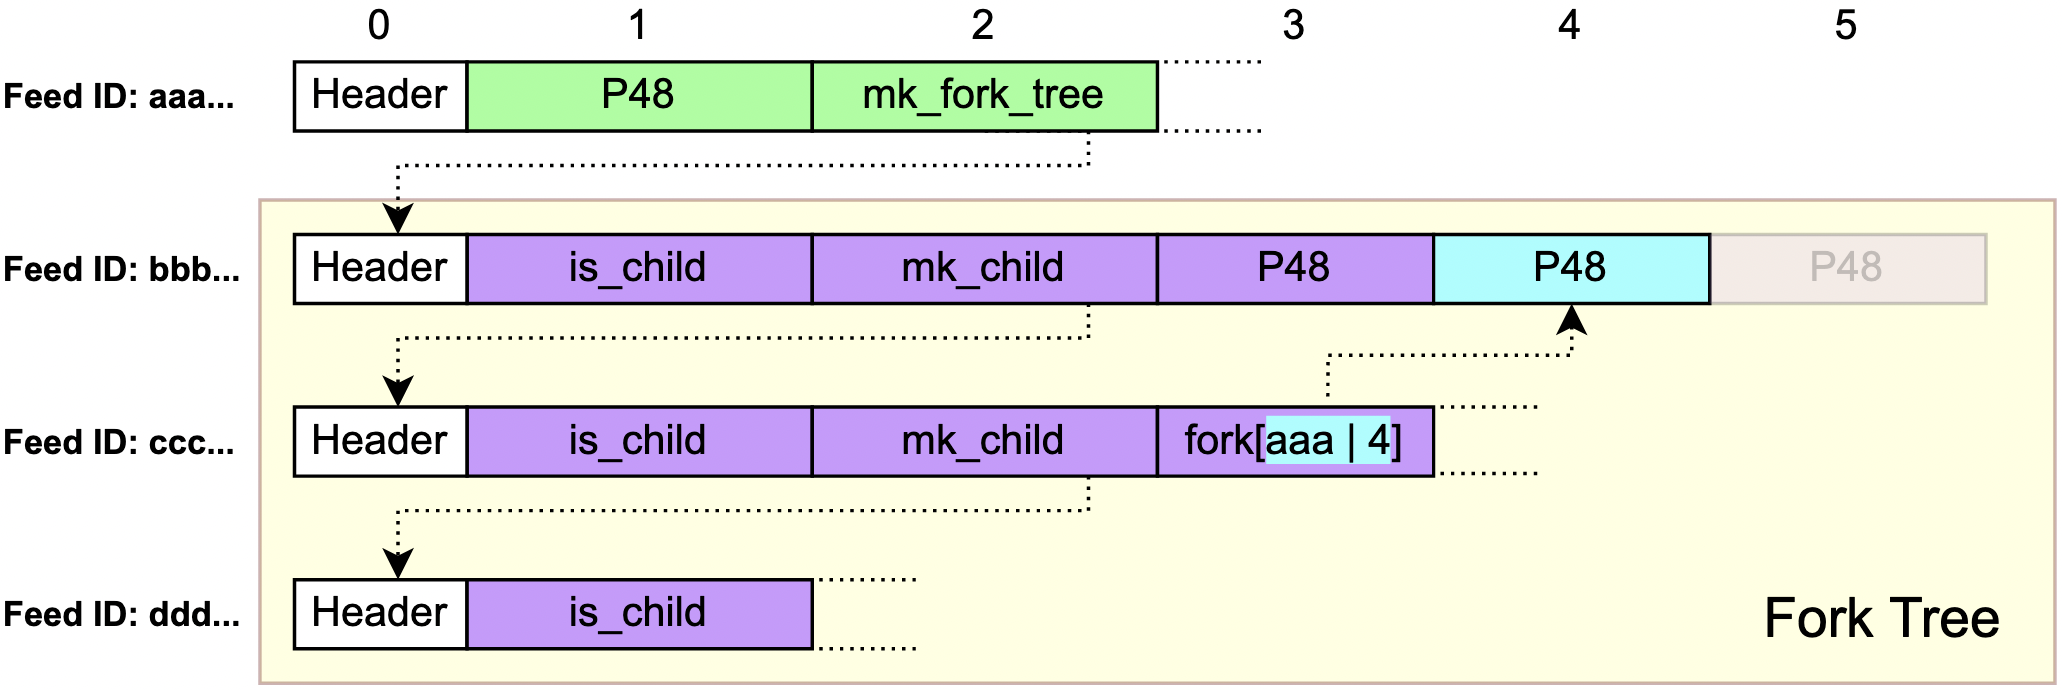
\includegraphics[width=1\textwidth]{fork2}
\caption{Fork Tree with one fork. The fork packet points to the new front packet in feed bbb... seq. nr. 4. Packet with seq. nr. 5 in feed bbb... is disregarded since it was added after the new front. No more packets can be appended to feed bbb... .}
\label{fig:fork2}
\end{figure}

A fork packet does not necessarily have to point to the previous feed. This is demonstrated in \cref{fig:fork3}. The second fork that was created in this example points to a packet before the first fork position. A fork can be created for any packet in the current packet chain except for the one in the front position (this would not revert any packets and only create an unnecessary additional feed).

\begin{figure}
\centering
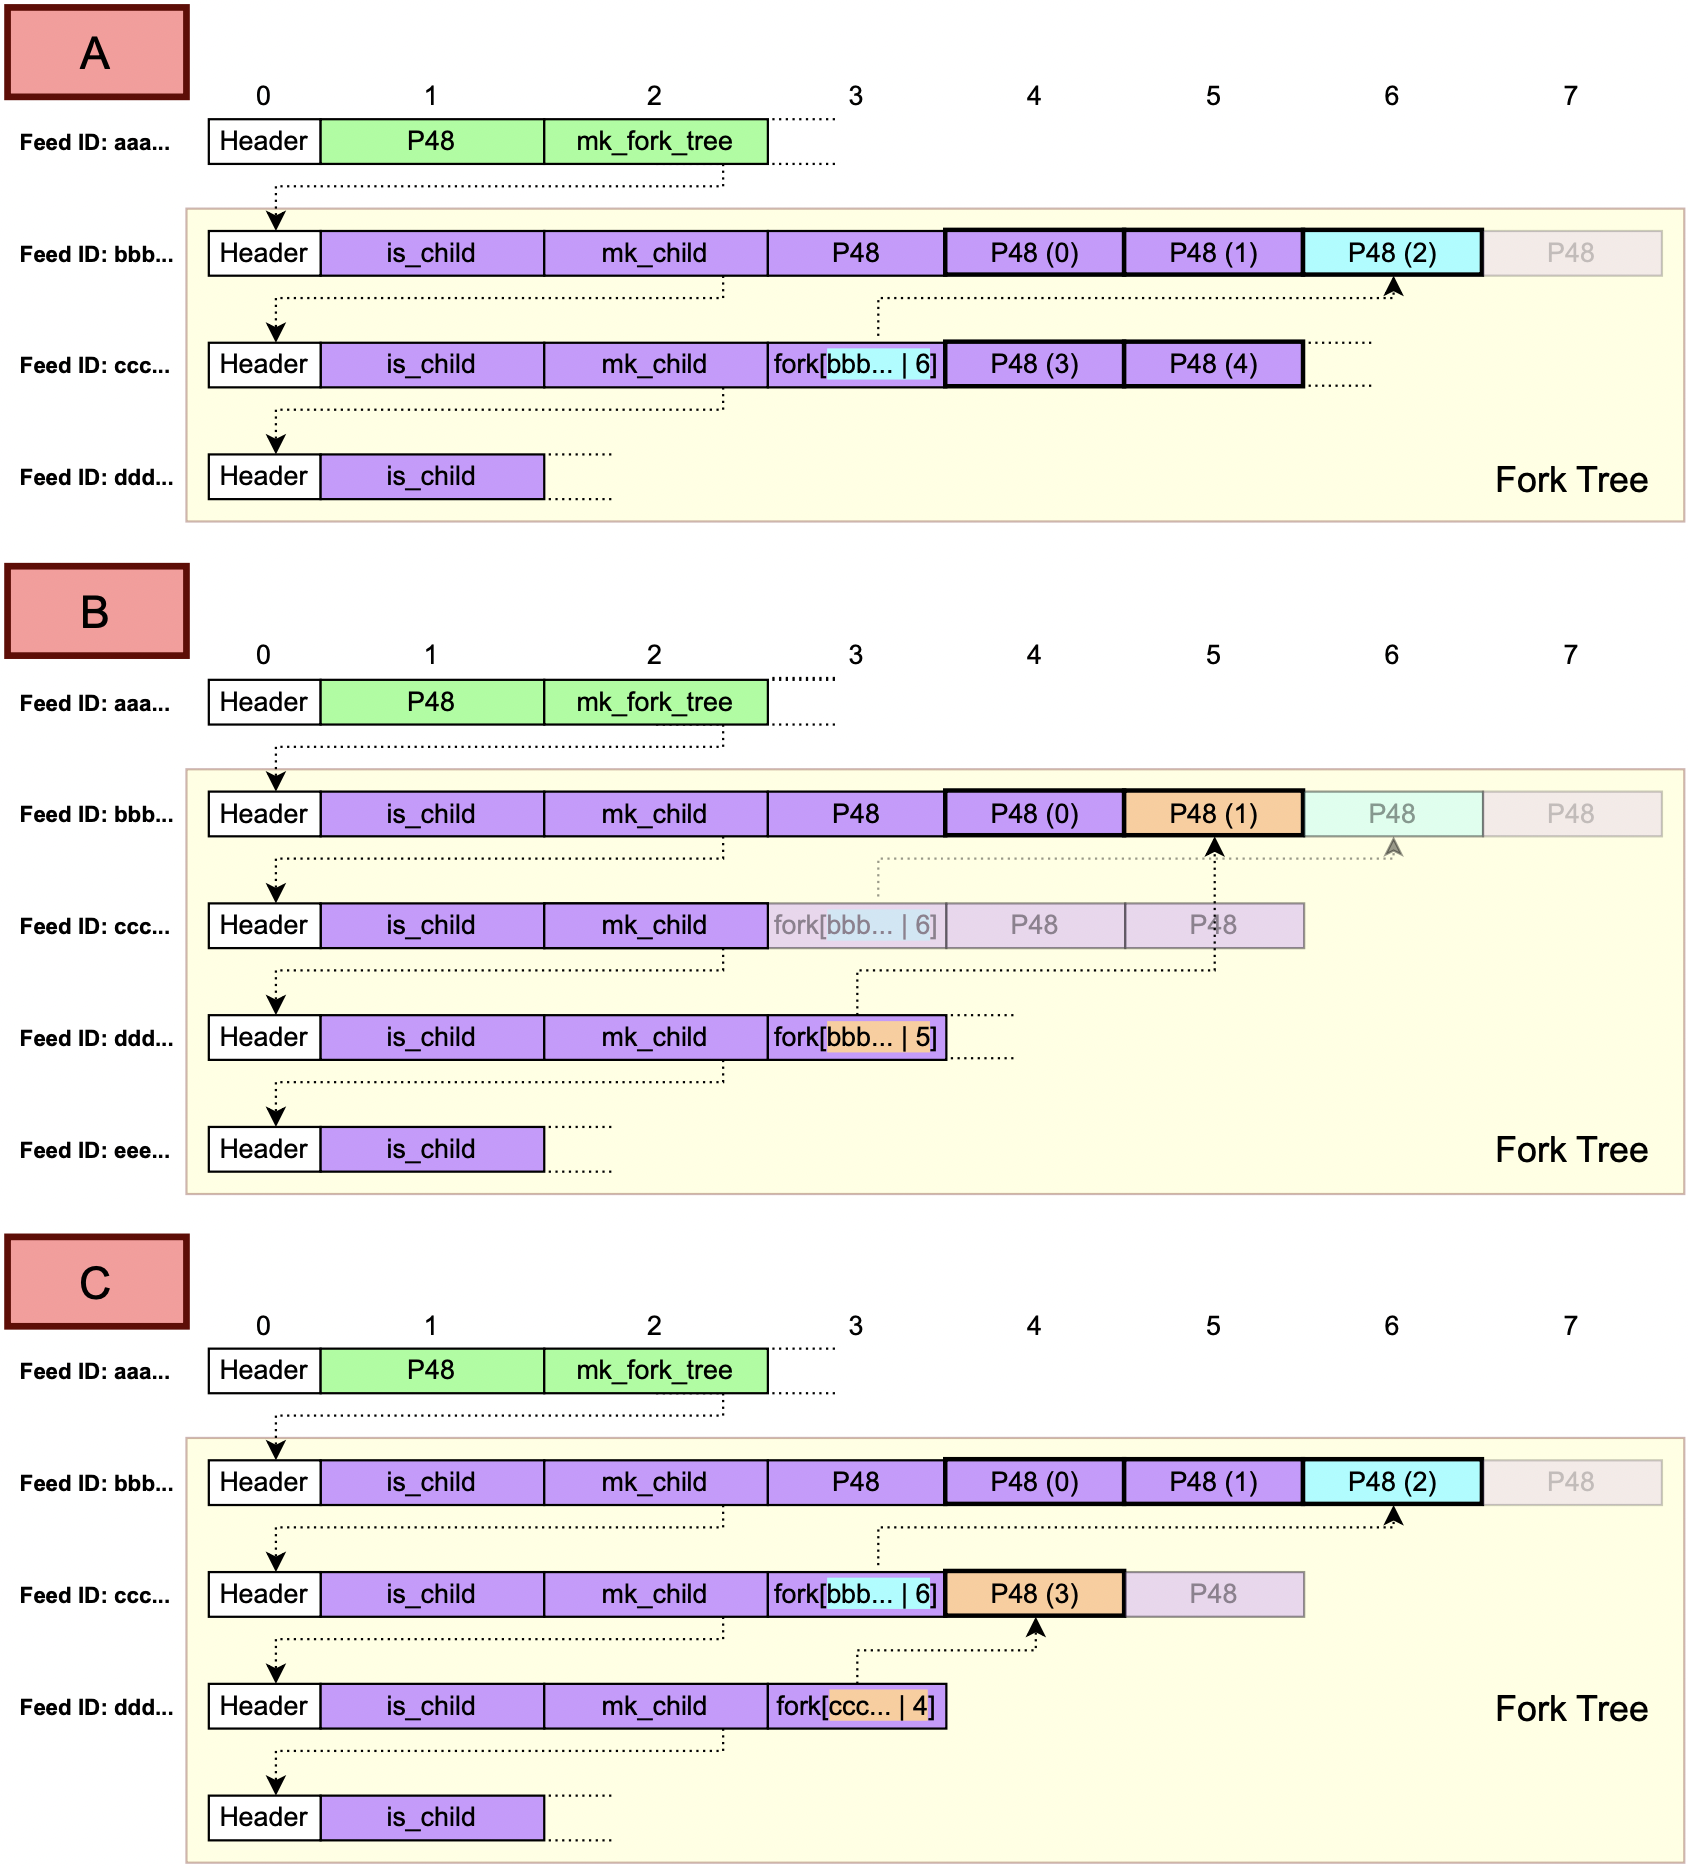
\includegraphics[width=1\textwidth]{fork3}
\caption{Fork Tree with one fork is presented in A. Packets with bold borders belong to the packet chain. The number in parenthesis describes their position in the chain. Transparent packets have been removed from the active tree by the forks. In B the same tree as in A with a new fork appended which points to an older version than the first fork is depicted. By forking a second time the last three packets are being dropped out of the chain and the first fork packet is not needed anymore. In C the tree from A is being forked at a newer position than the first fork.}
\label{fig:fork3}
\end{figure}


\subsection{Producer vs Consumer}
The functionalities discussed in \cref{sec:forking} mainly apply to the producer side\footnote{Node of the feed owner.}. On this side the newest state of the tree is always present, since it is created directly on the node without any transmission delays. However on the consumer side\footnote{Any Node that replicates the tree.} things get a little bit more complicated. The consumer slowly builds up the entire fork tree with packets received over the LoRa network. It is however not guaranteed, that the packets will be received in an optimal order. Situations may occur where a fork packet has already been received, but the packet it points to is not yet present in the tree. Therefore consumer nodes must after appending a packet to the tree always check if the tree is in its current state a valid fork tree. A fork tree is valid if \textbf{(1)} it has at least two feeds, \textbf{(2)} the last feed is set up as an emergency feed (only contains a header and a is-child packet) and \textbf{(3)} when starting at the newest packet and walking backwards along the fork pointers, every pointer points to a packet that exists in the tree. Tree validity does not guarantee that the tree is completely synchronized yet with the original producer tree but it guarantees that a valid readable packet chain can be deducted from its current state.

\subsection{Handling the DMX Values}
\label{sec:dmxfork}
DMX values only have to be inserted to the DMX table for consumer nodes. Producer nodes build the tree themselfs and do not need to request updates from other nodes.
After creating a lot of forks, the number of feeds contained in a fork tree can get large. If nodes would add a DMX value for every feed to the DMX table - and therefore request packets for every feed in the tree - a lot of effort would be used by the node to send want requests for only a single tree. To optimize this, feeds that are not used anymore can be removed from the DMX table. In fact the number of DMX values per fork tree can be reduced significantly. A DMX value for the current main feed and one for the emergency feed are needed at all times to be able to append new packets and to switch to a new fork if needed. If the tree is not valid yet, feeds that have not appended packets until the packet at the position they are forked, need to be added to the DMX table. If in \cite{fig:fork3} C feed bbb... had only appended packets until sequence number 3, the DMX value must stay in the table until the packet with sequence number 6 is appended. As soon as the forked position is appended, the DMX value can be removed for this feed.


\section{Session Tree}

\subsection{Feed Limitations}
\label{sec:sessionlimit}
Depending on the use-case of a TinySSB network, some nodes may accommodate feeds with a huge number of packets. To prevent them from filling the whole storage space on a device, at some point either no more packets can be appended or some older packets must be deleted. To prevent a node from adding data to a feed is rather undesirable since with not being able to add packets anymore it would essentially lock the node completely in its current state. Deleting older data is another approach which could work initially. However this would lead to problems when new nodes are deployed in the network or when some nodes - due to whatever complication - cannot reach the network for a longer period of time. When some packets in the chain are not available anymore, they cannot start or continue the trust chain (\cref{sec:anchor}) and therefore not reach the front of the feed. In this section a new approach called \textbf{session tree} that tackles this problem will be presented. The main idea is to split up the feed containing the payload into smaller continuation feeds and introduce new feeds that point to the payload feeds. A user defined number specifies the maximum number of payload feeds that must be stored. They all belong to the current session or sliding window. Once a new continuation feed is created, it is added to the sliding window and the oldest feed is removed from the sliding window. This lets the sliding window (session) move further in to the future while not changing its size. Consumer nodes can use the pointer feeds to reach the session and still keep a chain of trust.

\subsection{Initialization}
Analogously to initializing a fork tree, a new packet type 'make-session-tree' is introduced. After appending it to a feed, TinySSB creates a child feed that will be interpreted as a session tree root feed. Next a make-child packet must be appended to the root feed. This child feed represents the first session feed. A newly initialized session tree can be seen in \cref{fig:session1}. When the user appends payload packets to the session tree, they get appended here. The user can further manually specify how many payload packets should fit into one feed. After the feed has reached that number, a new continuation feed will be created. 

\begin{figure}
\centering
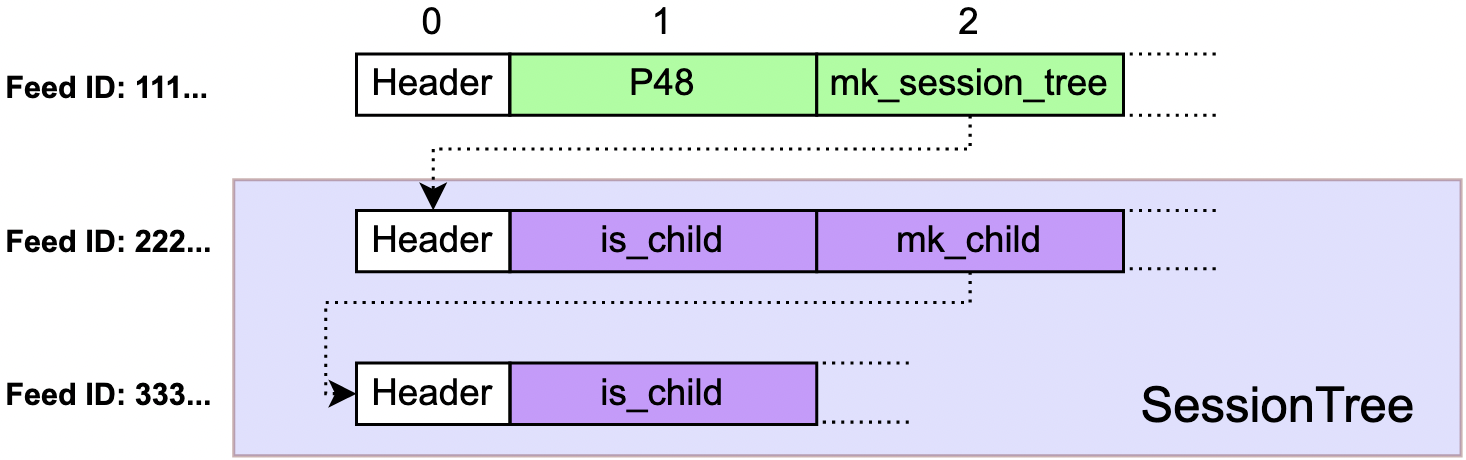
\includegraphics[width=1\textwidth]{session1}
\caption{A session tree initialized by the make-session-tree packet in feed 111... . Feed 222... is the root feed and feed 333... the first session feed where packets initially get appended to.}
\label{fig:session1}
\end{figure}

\subsection{Pointer Feeds}
Once the maximum number of packets is reached for the newest session feed, a continuation feed is created. All packets that are appended later get added to the continuation feed. Considering that in the future at some point the first session feed may be deleted, the session tree must find a way to still be able to access its continuation. To achieve that, a packet containing the feed ID of the continuation feed is appended to a pointer feed. If no pointer feed exists yet in the session tree, a new one will be initialized as a child feed of the root feed. (See \cref{fig:session2})

\begin{figure}
\centering
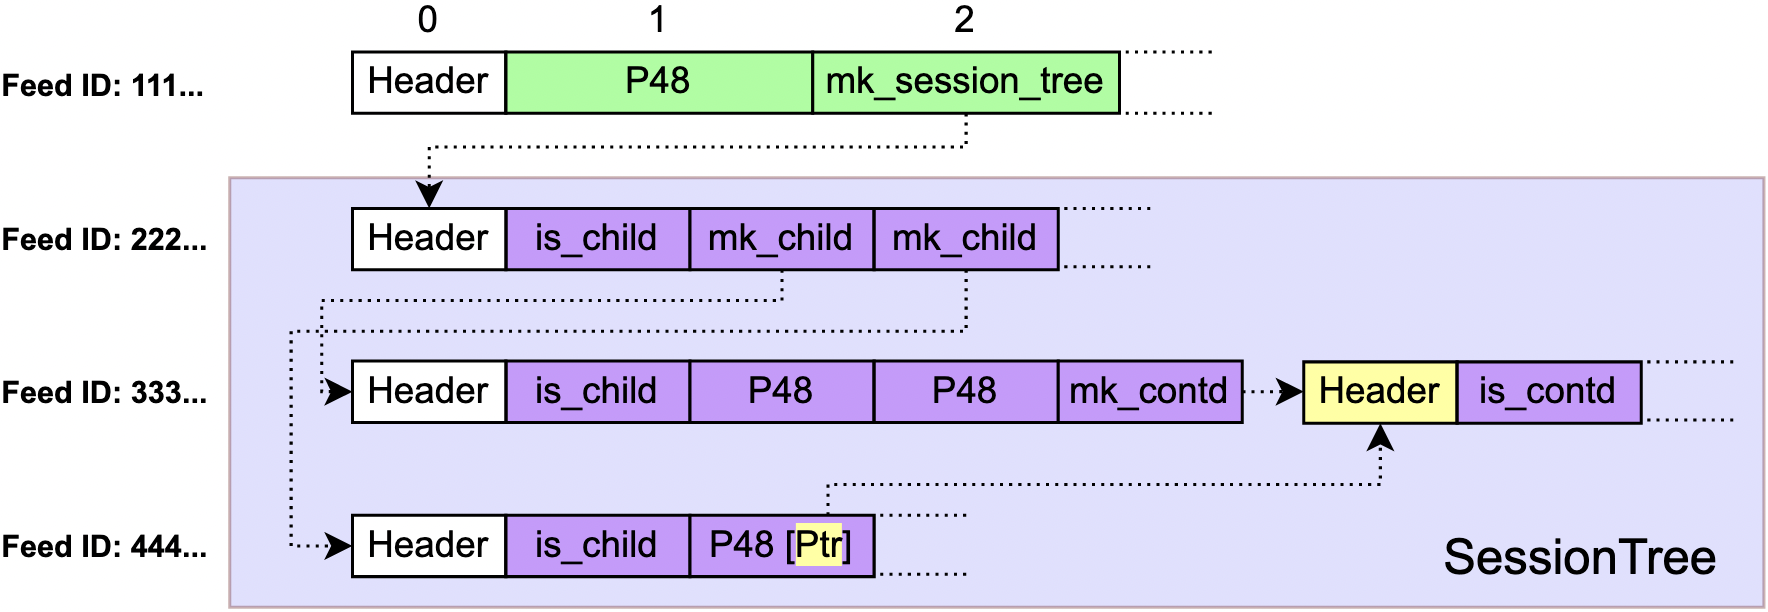
\includegraphics[width=1\textwidth]{session2}
\caption{A session tree with maximum payload packet per feed set to two. After two packets are appended, a continuation feed of the session feed 333... is created. A packet pointing to this continuation feed is added to the pointer feed 444... .}
\label{fig:session2}
\end{figure}

The session tree seen in \cref{fig:session2} has a pointer feed that grows slower than the session feed. However the problem stated in \cref{sec:sessionlimit} still remains. If the pointer feed grows too fast, limited storage space can still be filled rapidly by a session tree. To further optimize session trees and therefore adapt it to more use-cases, the same concept that is used for the session feeds can also be applied to the pointer feeds. When a pointer feed reaches the maximum number of pointers per feed, a continuation feed is created. To still keep track of all pointer feeds, a second layer of pointer feeds is created which points to the first layer of pointer feeds. The session tree can now grow in two dimensions. Horizontally it can create continuation feeds and vertically it can add more layers of pointer feeds. A new layer is created by adding a child feed to the root feed. 

\begin{figure}
\centering
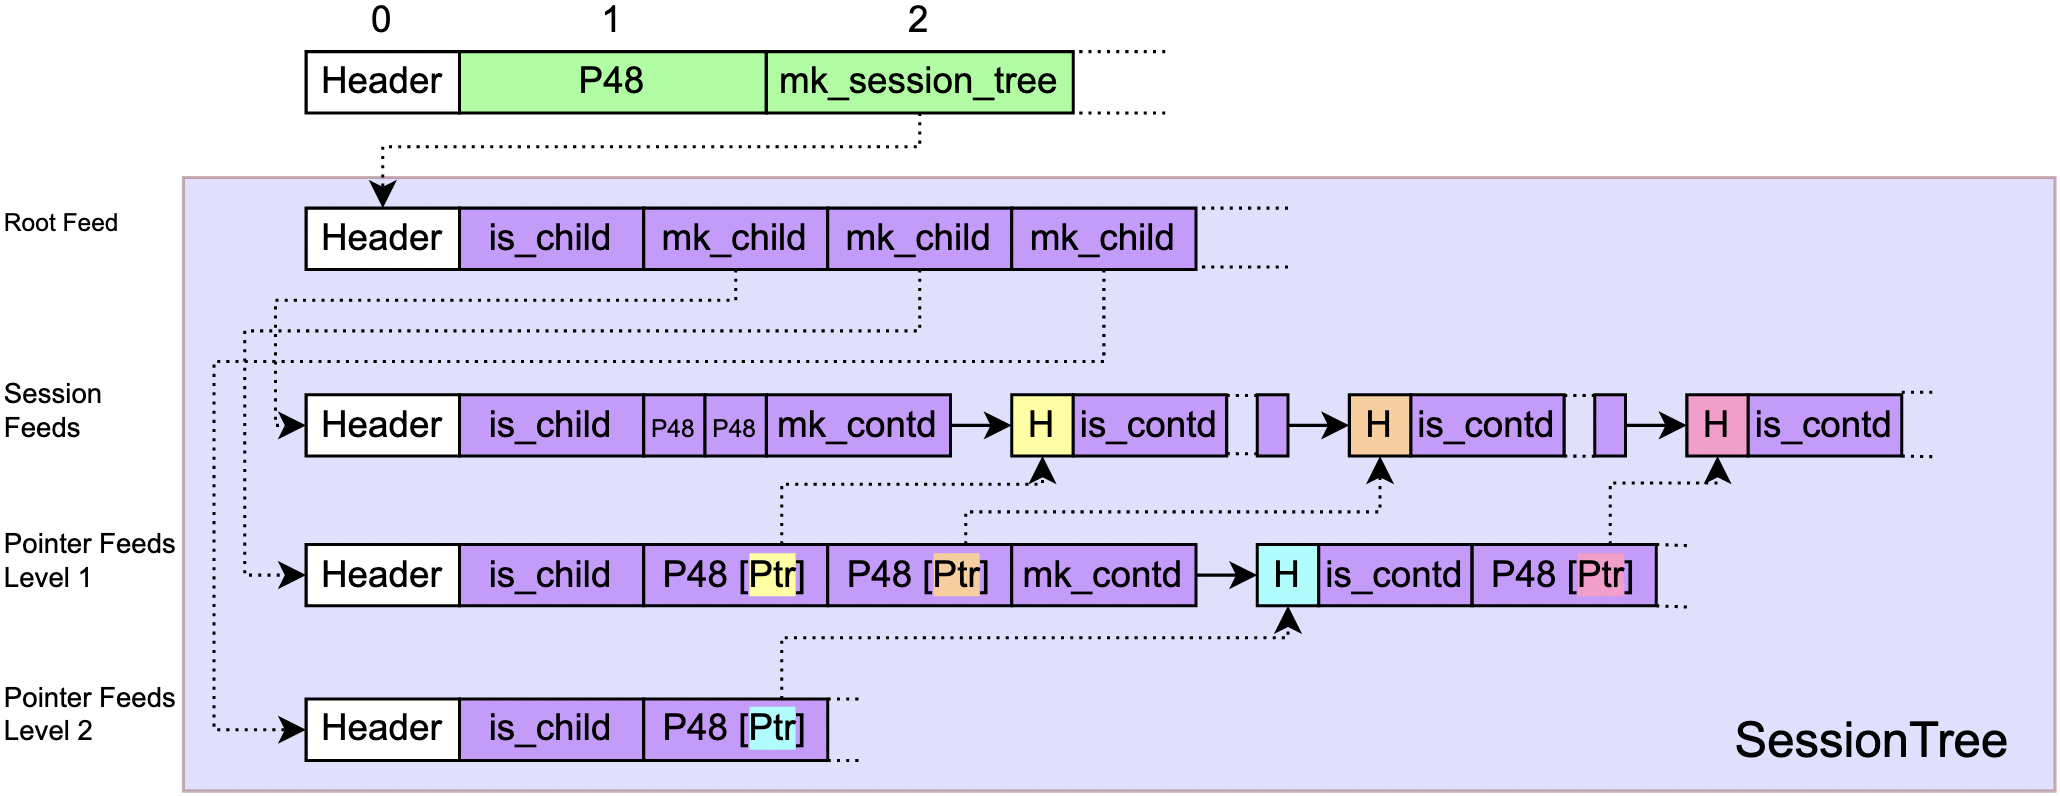
\includegraphics[width=1\textwidth]{session3}
\caption{A session tree with maximum two payload packet per feed. It contains four session feeds, two layer 1 pointer feeds with a total of three pointers and one layer 2 pointer feed.}
\label{fig:session3}
\end{figure}



\subsection{Producer vs Consumer}
As already seen in the fork tree case, the implementation of the producer side is much more straight foreword than the one of the consumer side. Every time a packet gets appended on the producer side, it gets appended to the newest session feed. If the feed has already the maximum number of packets, a continuation feed is created. If a new continuation feed had to be created, the node builds a packet that points to this new feed and appends it to the newest pointer feed on layer 1. If a continuation feed has to be created on this layer, again a packet that points to the new continuation feed gets created and appended one layer above. This is repeated until either no continuation feed has to be created anymore or the layer does not exist yet. If it does not yet exist, it the new layer gets created by appending a child feed to the root feed of the session tree and the last pointer packet is appended to the new layer. This algorithm is implemented in an iterative way. \\
On the consumer side things are different. No packets have to be appended manually. For every make-child packet in the root feed, the consumer creates a new feed (each representing the first feed in a session / pointer layer). If a pointer packet to a feed continuation is received and this feed is not yet created on the receiver side, it gets created even if its previous feed is not present. Every time a packet gets appended to the tree, the consumer updates the tree structure. If it can reach a new session feed via the pointer feeds (e.g. in \cref{fig:session3} on layer 2 blue pointer to layer 1, then red pointer to session feed with red marked header) it tries to load all its previous feeds until the user defined maximum number of session feeds is reached (if this number is 3, in \cref{fig:session3} first the previous feed with the orange header and then the previous feed with the yellow header is loaded if possible).


\subsection{Handling the DMX Values}
The consumer always has only the newest pointer feed per layer in the DMX table. If the user specified that a maximum of n session feeds can be stored on the device, 0 to n session feed DMX values can be in the DMX table. As soon as a continuation is created in any layer, the DMX table gets updated and only the newest feed will be present in the table. Since the consumer does not know if it has already received the newest pointer layer, it has to keep requesting packets for the root feed and the pointer feeds. Optimizing the requesting of session feed packets is something that needs to be further looked into in the future and that may reduce storage and time overhead that still exists in the current implementation. [ADD REF]
